\documentclass{beamer}
 
\usepackage[utf8]{inputenc}
\usepackage[T1]{fontenc}
%\usepackage{babel}
\usepackage{hyperref}

\setbeamertemplate{footline}[frame number]
\AtBeginSection[]
{
  \begin{frame}
    \frametitle{Table of Contents}
    \tableofcontents[currentsection]
  \end{frame}
}
 
%Information to be included in the title page:
\title%optional
{Projet d'informatique III transdisciplinaire}
 
\subtitle{Chauffage intelligent}
 
\author[Sacha Medaer, Nicolas Feron, Nicolas Potvin, Kishiro Nishio] % (optional, for multiple authors)
{Sacha Medaer, Nicolas Feron, Nicolas Potvin, Kishiro Nishio}
 
 
\date
{Faculté des sciences, Décembre 2016}
 
\logo{
\includegraphics[height=1.5cm]{logo_ulb}}
 
 
\begin{document}
 
\frame{\titlepage}

\begin{frame}
\frametitle{Table des matières}
\tableofcontents
\end{frame}
 
\section{Introduction}
 
\begin{frame}
\frametitle{Présentation}
 \begin{block}{But}
 	Développer une application android qui décide de manière autonome quand et comment chauffer les pièces d'une maison
 \end{block}
 \vspace{10 mm}
 2 parties:
 \begin{itemize}
 \item client
 \item serveur
 \end{itemize}
\end{frame}

\begin{frame}
\frametitle{Cahier des charges}
L'application doit dépendre de :
\begin{itemize}
\item historique des modifications manuelles
\item habitude des membres de la famille 
\item positions des membres de la famille
\item conditions météorologiques
\end{itemize}
N.B.: l'utilisateur peut également changer manuellement le chauffage
\end{frame}

\section{Base de données}
\begin{frame}
\frametitle{Schéma Entités-Relations}
\begin{center}
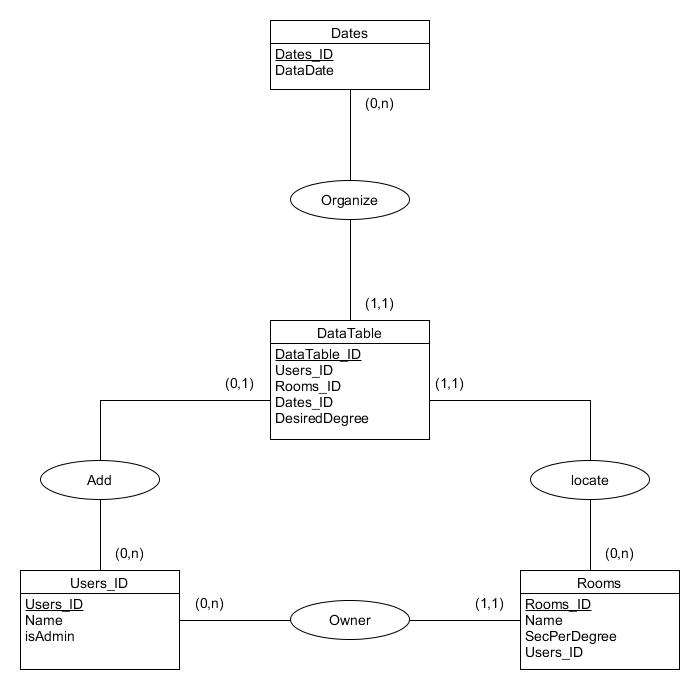
\includegraphics[scale=0.35]{DataBase}
\end{center}
\end{frame}

\section{Diagramme UML}
\begin{frame}
\frametitle{Diagramme de classes}
\begin{center}
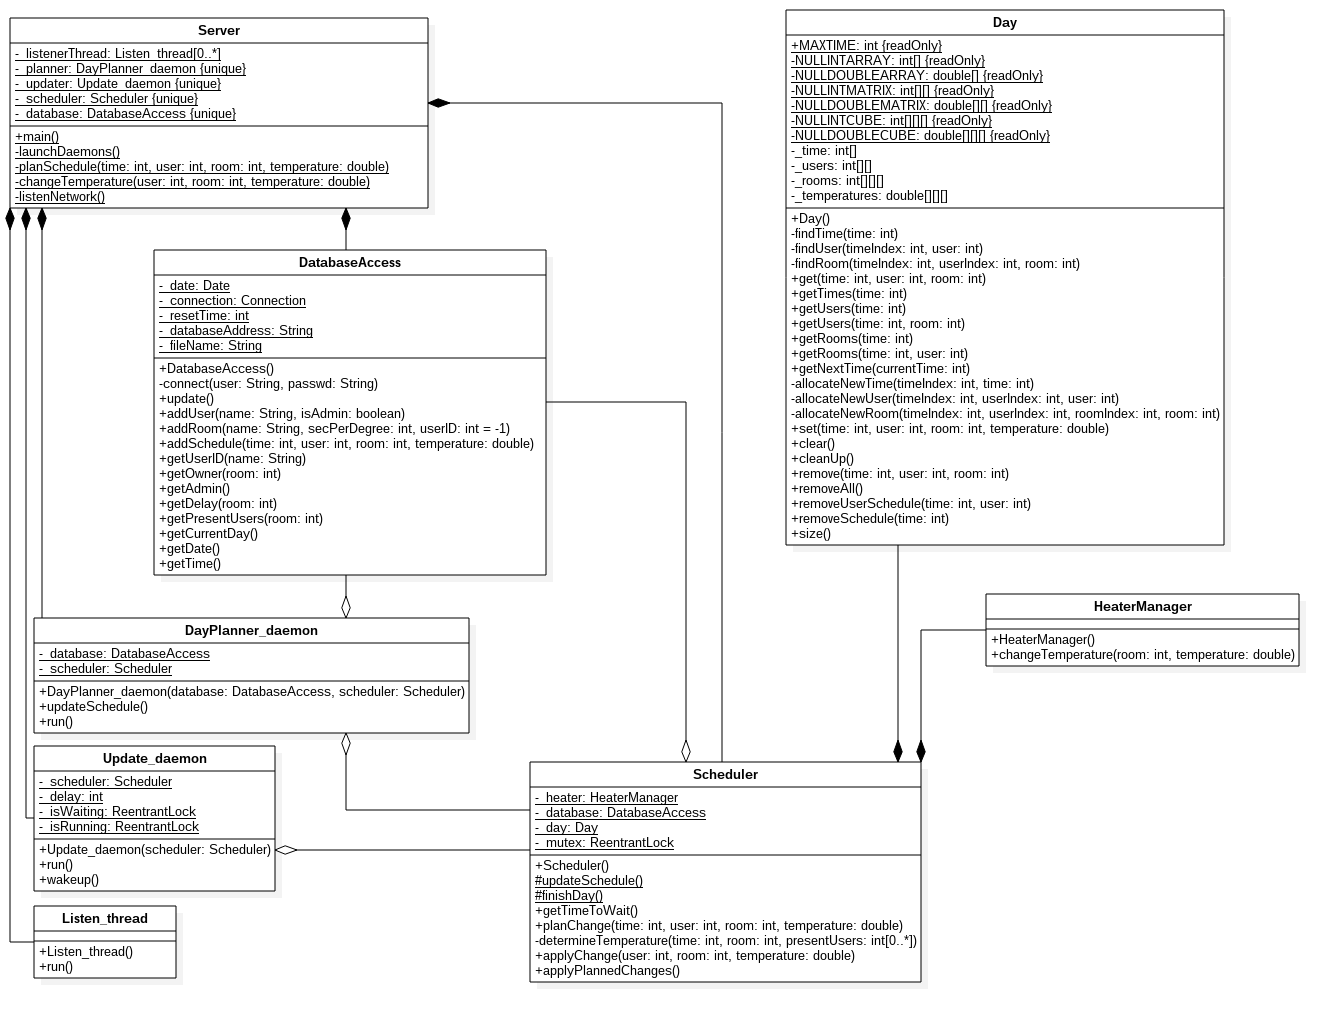
\includegraphics[scale=0.22]{classdiaSERVER}
\end{center}
\end{frame}

\section{Apprentissage autonome}
\subsection{Introduction}
\begin{frame}
\frametitle{Machine learning}
%\begin{alertblock}{Data mining}
%déduction d'un modèle à partir d'un ensemble de données, fondation pour l'intelligence artificielle et le machine learning.
%\end{alertblock}
%\begin{alertblock}{Artificial Intelligence}
%algorithmes qui s'adonnent à des tâches qui demandent des processus mentaux d%e haut niveau.
%\end{alertblock}
\begin{alertblock}{Définition}
algorithmes qui permettent à une machine d'évoluer son comportement de manière autonome à partir de données empiriques.
\end{alertblock}
\end{frame}

%\begin{frame}
%$\longrightarrow$ pas de hiérarchie, les 3 en symbiose 
%\begin{center}
%\begin{figure}[!h]
%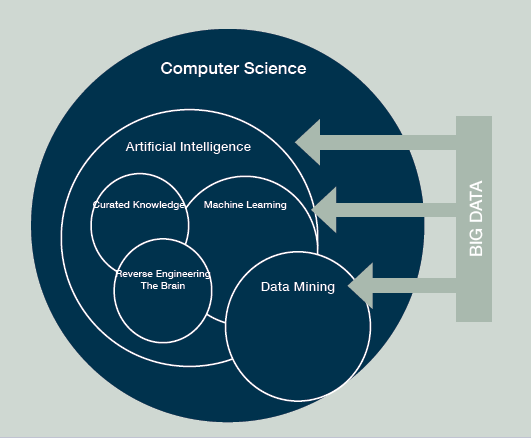
\includegraphics[scale=0.4]{bigdata_graph}
%\caption{\url{inovancetech.com/buzzwords.html}}
%\end{figure}
%\end{center}
%\end{frame}

\begin{frame}
\frametitle{2 types principaux de machine learning}
\begin{itemize}
\item \huge Unsupervised learning
\item \huge Supervised learning
\end{itemize}
\end{frame}

\begin{frame}
\frametitle{Méthodes de machine learning}
\begin{itemize}
\item Anomaly detection
\item Association rule mining
\item \textbf{Clustering}
\item \textbf{Classification}
\item Regression
\item Summarization
\end{itemize}
\end{frame}

\subsection{Et pour notre application?}
\begin{frame}
\frametitle{Clustering}
\begin{alertblock}{Définition}
Division d'un ensemble en sous-ensembles en fonction des affinités des éléments qui le compose.
\end{alertblock}
\begin{itemize}
\item unsupervised learning
\item analyse statistique de données
\end{itemize}
\end{frame}

\begin{frame}
\frametitle{Classification (logistic regression)}
\begin{alertblock}{Définition}
Identification de la catégorie (connue) à laquelle un nouvelle élément appartient en se basant sur l'observation d'un training set.
\end{alertblock}
\begin{itemize}
\item supervised learning
\item analyse statistique de données
\end{itemize}
\end{frame}

\section{Conclusion}

\begin{frame}
\frametitle{Où en est-on ?}
\begin{itemize}
  \item Code du serveur presque fini
  \item Base de données terminée
  \item Idées concernant le machine learning
\end{itemize}
\end{frame}

\begin{frame}
\frametitle{Ce qu'il nous reste à faire}
\begin{itemize}
  \item Le code de l'application
  \item L'implémentation du machine learning
  \item trouver comment lier le hardware du chauffage avec le serveur
\end{itemize}
\end{frame}

\begin{frame}
\frametitle{Printemps des Sciences}
\begin{itemize}
  \item Vulgarisation des concepts
  \item Idée de présentation interactive ("maison de poupée" si possible)
  \item Intéresser les gens : Le Machine Learning, c'est cool !
\end{itemize}
\end{frame}

\begin{frame}
\huge Questions
\end{frame}	
 
\end{document}
